% Original book diagram: fig:concept_map
% Book source: sections/front/preface.tex
% Original diagram authorship retained. Visual design: Ziad Mosalam.
\documentclass[11pt,border=8pt]{standalone}
\usepackage{amsmath,amssymb,graphicx,tikz}
\usetikzlibrary{arrows.meta,automata,positioning,calc,shapes.geometric,fit,backgrounds,patterns}
\newcommand{\vect}[1]{\mathbf{#1}}
\newcommand{\mat}[1]{\mathbf{#1}}
\newcommand{\Normal}{\mathcal{N}}
\newcommand{\prob}{p}
\newcommand{\E}{\mathbb{E}}
\newcommand{\Var}{\mathrm{Var}}
\newcommand{\Cov}{\mathrm{Cov}}
\newcommand{\CovP}{\mathbf{P}}
\newcommand{\Prob}{\mathbb{P}}
\setlength{\textwidth}{6.5in}
% Shared visual vocabulary for the book's original diagrams.
% Figures opt in explicitly, so unrelated text and existing additions are unchanged.
\definecolor{BookBlue}{HTML}{003262}
\definecolor{BookGold}{HTML}{B17A00}
\definecolor{BookTeal}{HTML}{247C86}
\definecolor{BookInk}{HTML}{30363B}
\definecolor{BookLight}{HTML}{E9EFF5}
\tikzset{
  book figure/.style={font=\small\rmfamily, color=BookBlue, text=BookInk,
    line width=0.8pt, >=Latex},
  book axis/.style={->, draw=BookInk, line width=0.6pt},
  book link/.style={->, draw=BookBlue, line width=0.8pt},
  book observation/.style={draw=BookGold, fill=BookGold!8},
  book state/.style={draw=BookBlue, fill=BookLight},
  book note/.style={font=\footnotesize\rmfamily, text=BookInk}
}

\begin{document}
\resizebox{\textwidth}{!}{%
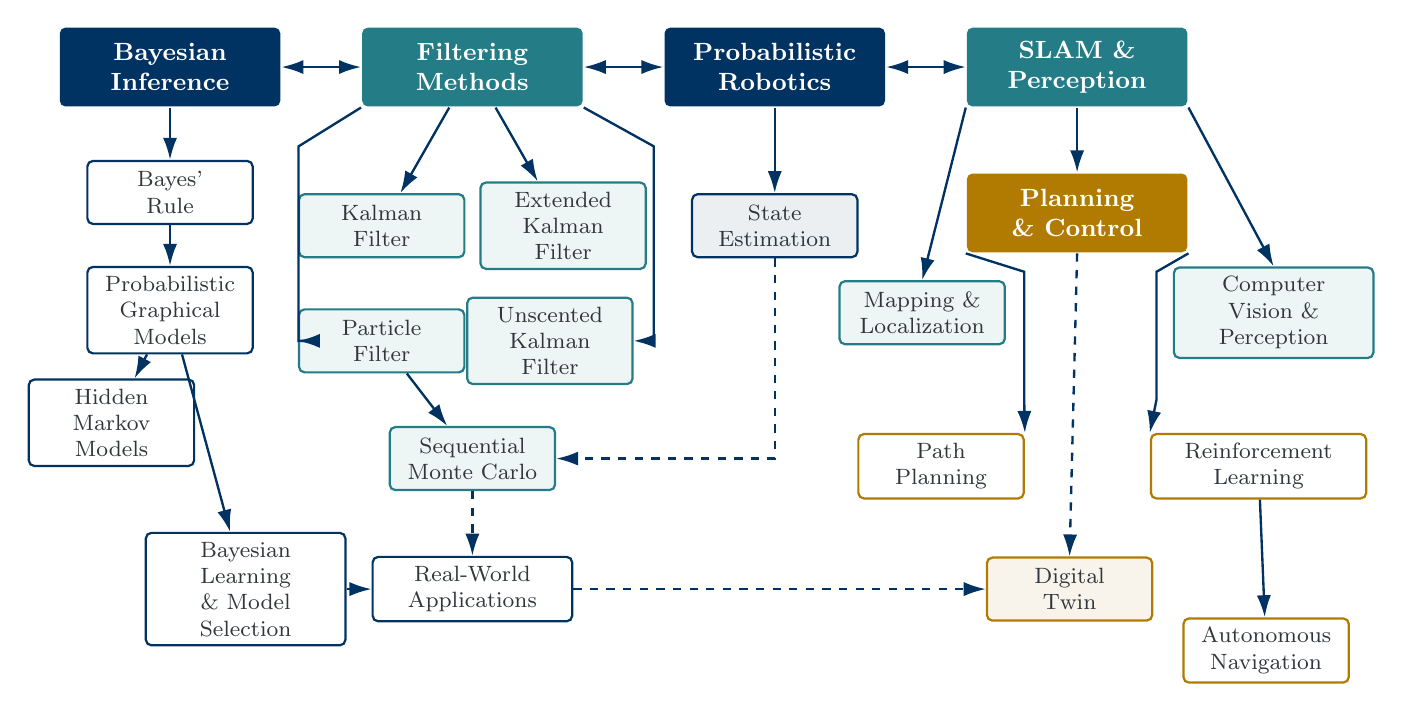
\begin{tikzpicture}[book figure, x=0.48cm, y=0.65cm,
    >= {Latex[length=2.8mm,width=1.8mm]},
    main/.style={rectangle,rounded corners=2pt,draw=none,minimum width=2.8cm,minimum height=1.0cm,font=\small\rmfamily\bfseries,text=white,align=center},
    sub/.style={rectangle,rounded corners=2pt,draw,minimum width=2.1cm,text width=1.85cm,minimum height=0.8cm,font=\footnotesize\rmfamily,align=center},
    arrow/.style={-{Latex[length=2.8mm,width=1.8mm]},line width=0.85pt},
    top link/.style={{Latex[length=2.8mm,width=1.8mm]}-{Latex[length=2.8mm,width=1.8mm]},line width=0.85pt},
    secondary/.style={arrow,dashed}
]
\colorlet{myorange}{BookBlue}
\colorlet{mygreen}{BookTeal}
\colorlet{myblue}{BookBlue}
\colorlet{mypurple}{BookTeal}
\colorlet{myred}{BookGold}

% Major themes are placed at identical y-coordinates.
\node[main,fill=myorange] (bayes) at (0,0) {Bayesian\\Inference};
\node[main,fill=mygreen] (filter) at (8,0) {Filtering\\Methods};
\node[main,fill=myblue] (prob) at (16,0) {Probabilistic\\Robotics};
\node[main,fill=mypurple] (slam) at (24,0) {SLAM \&\\Perception};
\node[main,fill=myred] (plan) at (24,-2.85) {Planning \\\& Control};

% Inference and learning.
\node[sub,draw=myorange] (bayesrule) at (0,-2.45) {Bayes'\\Rule};
\node[sub,draw=myorange] (pgm) at (0,-4.75) {Probabilistic\\Graphical Models};
\node[sub,draw=myorange] (hmm) at (-1.55,-6.95) {Hidden\\Markov Models};
\node[sub,draw=myorange,minimum width=2.5cm,text width=2.3cm] (learn) at (2,-10.2) {Bayesian Learning\\\& Model Selection};

% Filtering methods, including both nonlinear Kalman filters.
\node[sub,draw=mygreen,fill=mygreen!8] (kf) at (5.6,-3.1) {Kalman\\Filter};
\node[sub,draw=mygreen,fill=mygreen!8] (ekf) at (10.4,-3.1) {Extended\\Kalman Filter};
\node[sub,draw=mygreen,fill=mygreen!8] (pf) at (5.6,-5.35) {Particle\\Filter};
\node[sub,draw=mygreen,fill=mygreen!8] (ukf) at (10.05,-5.35) {Unscented\\Kalman Filter};
\node[sub,draw=mygreen,fill=mygreen!8] (smc) at (8,-7.65) {Sequential\\Monte Carlo};

% State estimation and perception.
\node[sub,draw=myblue,fill=myblue!8] (state) at (16,-3.1) {State\\Estimation};
\node[sub,draw=mypurple,fill=mypurple!8] (map) at (19.9,-4.8) {Mapping \&\\Localization};
\node[sub,draw=mypurple,fill=mypurple!8,minimum width=2.5cm,text width=2.3cm] (vision) at (29.2,-4.8) {Computer \\ Vision \& \\ Perception};

% Planning and applications.
\node[sub,draw=myred] (path) at (20.4,-7.8) {Path\\Planning};
\node[sub,draw=myred,minimum width=2.7cm,text width=2.5cm] (rl) at (28.8,-7.8) {Reinforcement\\Learning};
\node[sub,draw=myred] (nav) at (29.0,-11.4) {Autonomous\\Navigation};
\node[sub,draw=myred,fill=myred!8] (dt) at (23.8,-10.2) {Digital\\Twin};
\node[sub,minimum width=2.5cm,text width=2.3cm] (apps) at (8,-10.2) {Real-World\\Applications};

% Exactly horizontal double-headed conceptual connections.
\draw[top link] (bayes.east) -- (filter.west);
\draw[top link] (filter.east) -- (prob.west);
\draw[top link] (prob.east) -- (slam.west);

% Hierarchical and methodological links.
\draw[arrow] (bayes) -- (bayesrule);
\draw[arrow] (bayesrule) -- (pgm);
\draw[arrow] (pgm) -- (hmm);
\draw[arrow] (pgm) -- (learn);
\draw[arrow] (filter) -- (kf);
\draw[arrow] (filter) -- (ekf);
\draw[arrow] (filter.south west) -- (3.4,-1.55) -- (3.4,-5.35) -- (pf.west);
\draw[arrow] (filter.south east) -- (12.8,-1.55) -- (12.8,-5.35) -- (ukf.east);
\draw[arrow] (pf) -- (smc);
\draw[arrow] (prob) -- (state);
\draw[arrow] (slam.south west) -- (map.north);
\draw[arrow] (slam.south east) -- (vision.north);
\draw[arrow] (slam.south) -- (plan.north);
\draw[arrow] (plan.south west) -- (22.6,-4.0) -- (22.6,-6.5) -- (path.north east);
\draw[arrow] (plan.south east) -- (26.1,-4.0) -- (26.1,-6.5) -- (rl.north west);
\draw[arrow] (rl) -- (nav);

% Secondary / cross-cutting / application links.
\draw[secondary] (smc) -- (apps);
\draw[secondary] (learn.east) -- (apps.west);
\draw[secondary] (state.south) -- (16,-7.65) -- (smc.east);
\draw[secondary] (plan.south) -- (dt.north);
\draw[secondary] (apps.east) -- (dt.west); % horizontal: matching node center heights
\end{tikzpicture}%
}
\end{document}
